\chapter{Results and Discussion}
\label{ch:Results-and-Discussion}
Following the brief example demonstration of the proposed method in Chapter \ref{ch:Methodology}, we extended the implementation to house 12 of the \gls{refit} data set. The subsequent sections serve to demonstrate the efficacy of both the classification step as well as the forecasting step of our proposed method. 

\section{Cluster Label Classification}
\label{sec:Results-and-Discussion:Cluster-Label-Classification}
The first results that we will be demonstrating are that of the classification step of our proposed method -- refer to Table \ref{tab:Classification-results}.

\begin{table}[H]
        \myfloatalign
        \centering
        \begin{tabular*}{\linewidth}{c@{\extracolsep{\fill}}c@{\extracolsep}c} \toprule
                \tableheadline{Data Set} & \tableheadline{No. of Clusters} & \tableheadline{Accuracy} \\ \midrule
                \gls{ucid}               & 3                               & 76\%                     \\ \midrule
                \gls{refit} - House 12   & 3                               & 66\%                     \\ \bottomrule
        \end{tabular*}
        \caption{Result of training, optimizing and evaluating a random forest classifier on the cluster labels obtained for each of the \gls{ucid} as well as the \gls{refit} data sets.}
        \label{tab:Classification-results}
\end{table}

\noindent \newline Being able to correctly assign new samples into the correct cluster is imperative so as to insure the highest likelihood of achieving consistently reliable forecasting accuracy. Given that we had an equal number of 3 clusters per data set and that we were working with a (synthetic) uniform distribution of samples over the different clusters; the scores outlined in Table \ref{tab:Classification-results} are fairly good (a random predictor would achieve an accuracy of 33.3\%). The disparity in the results between the 2 data sets could predominantly be linked to the following 2 reasons:

\begin{enumerate}
    \item The \gls{ucid} data set contained a much larger number of samples (days).
    \item The distribution of the samples over the different days of the week as well as the months is much more uniform in the \gls{ucid} data set (refer to Figures \ref{fig:REFIT-Distribution} and \ref{fig:UCID-Distribution} of Chapter \ref{ch:Exploratory-Data-Analysis}).
\end{enumerate}

\noindent \newline Figures \ref{fig:UCID-Classification-Confusion-Matrix} and \ref{fig:REFIT-Classification-Confusion-Matrix} allow us to clearly visualize both the correct as well as the incorrect predictions made by our model. Interestingly, given that both the clusters formed for each of the \gls{ucid} as well as the \gls{refit} data set were quite similar in terms of the overall patterns that were captured, the fitted model per data set seems to be making mistakes, or otherwise incorrect predictions, of a similar magnitude with cluster 2 containing the largest amount of incorrect predictions for each of the data sets and cluster 1 containing the largest amount of correct predictions.

\begin{figure}[H]
    \begin{adjustwidth}{-3.0cm}{-3.0cm}%
            \myfloatalign
            \subfloat[Confusion matrix - \gls{ucid}.]
            {
                    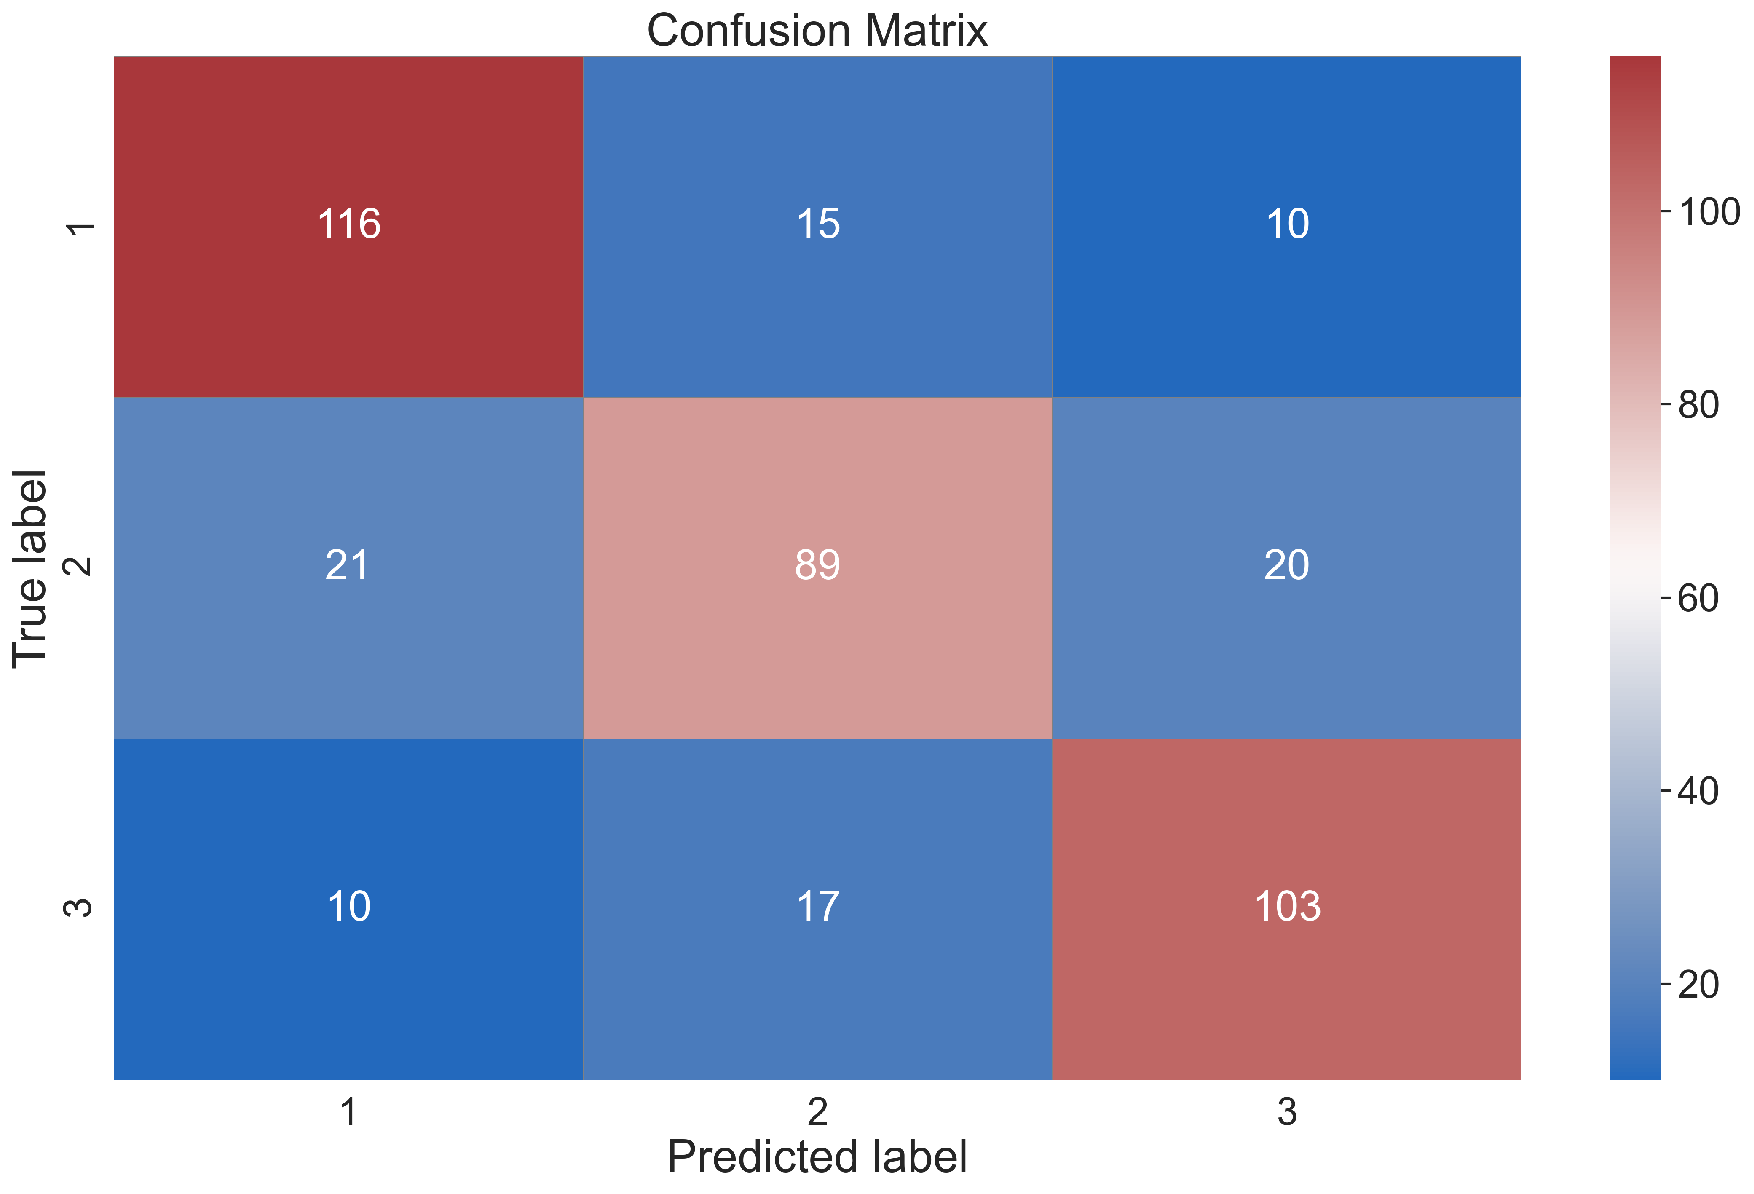
\includegraphics[width=0.7\textwidth]{Images/Chapter 7/UCID/UCID-Classification-Confusion-Matrix.pdf}
                    \label{fig:UCID-Classification-Confusion-Matrix}
            } \quad
            \subfloat[Confusion matrix - \gls{refit}.]
            {
                    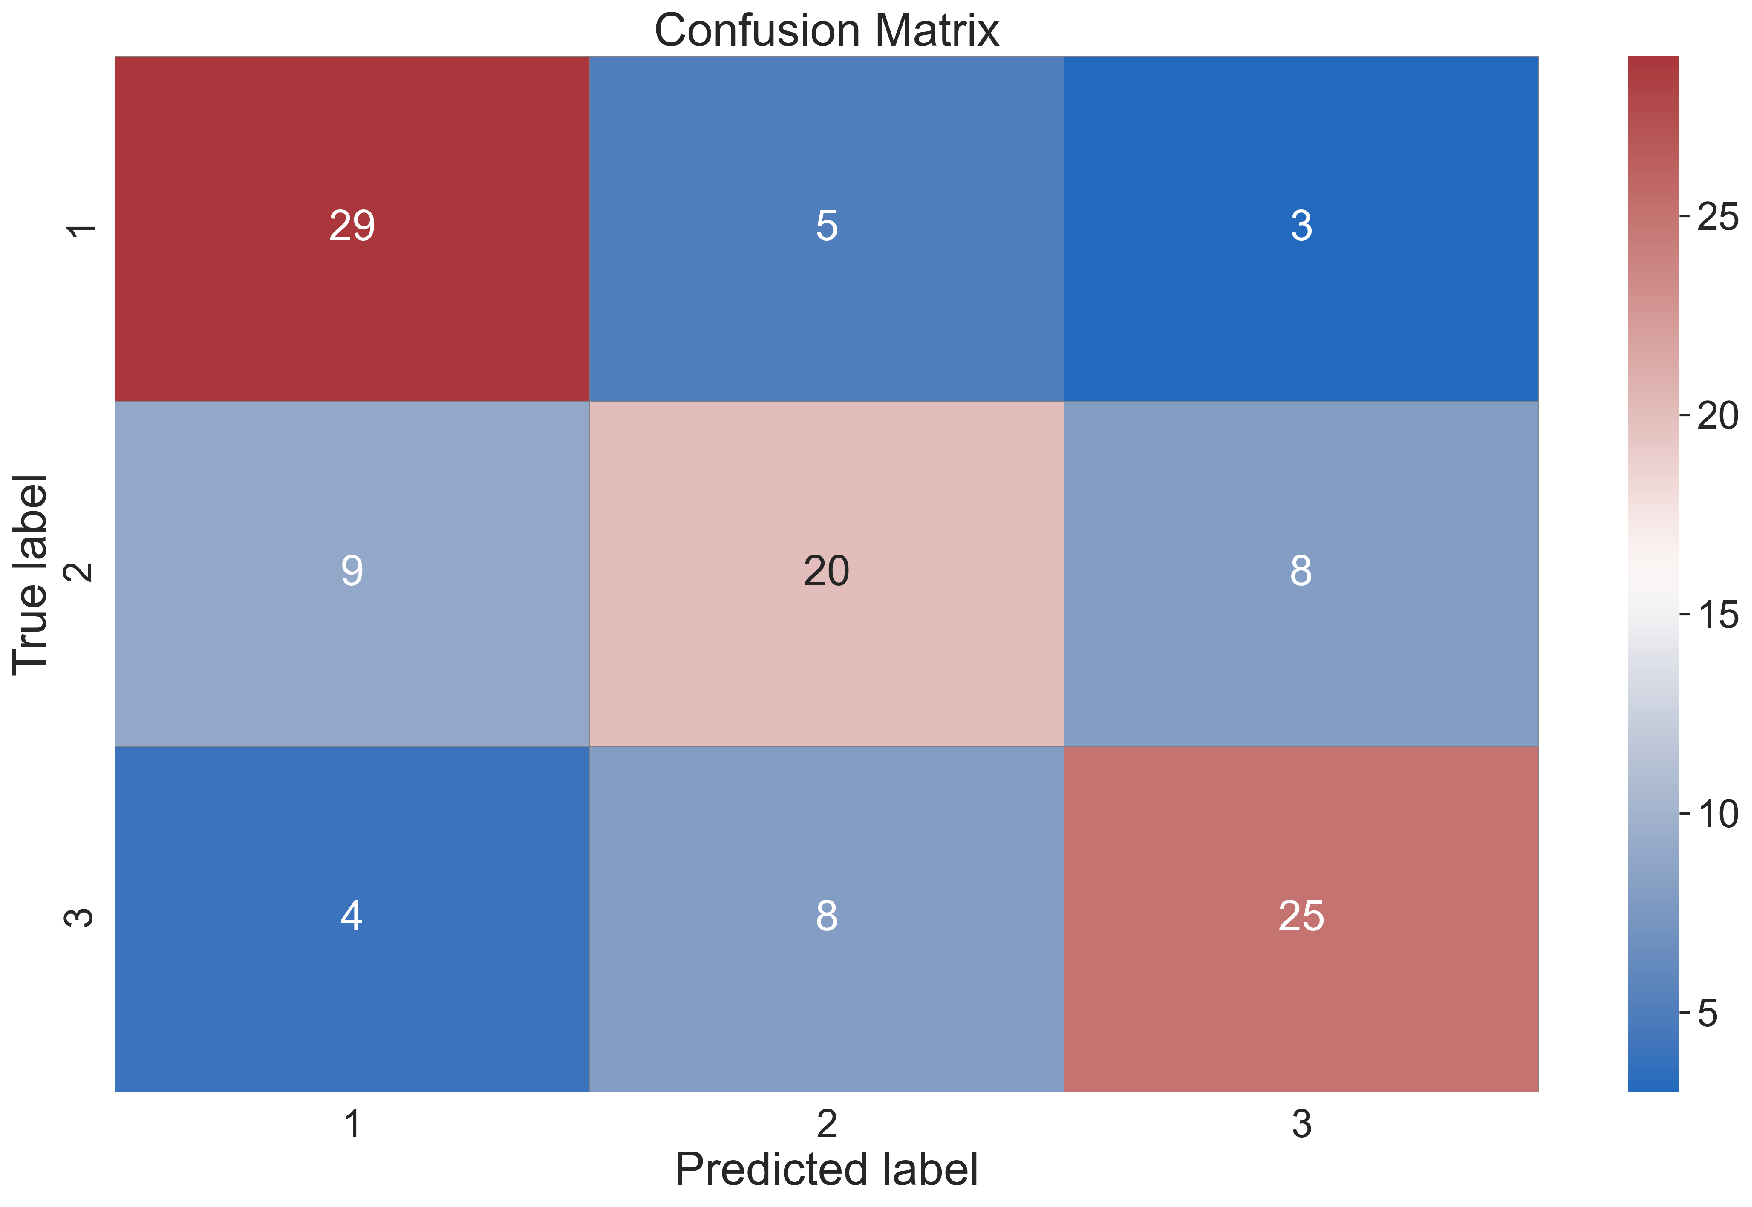
\includegraphics[width=0.7\textwidth]{Images/Chapter 7/REFIT/REFIT-Classification-Confusion-Matrix.pdf}
                    \label{fig:REFIT-Classification-Confusion-Matrix}
            } \quad
            \caption{Confusion matrices for each of the \gls{ucid} as well as the \gls{refit} data sets.}
    \end{adjustwidth}
\end{figure}

\noindent \newline One of the benefits of our proposed method that we previously discussed is that no prior knowledge of the number of clusters is required; as there is no guarantee that any 2 individual households contain a similar number of \textit{repeating} patterns we avoid running into the problem of overly generalizing a single working solution that may or may not work given said change in energy consumption patterns and instead present a solution that could potentially extend to a much larger scale. A potential issue with this implementation however, is that an individual household \textit{may} contain a large number of repeating consumption patterns which could possibly lead to an overall decline in what can already be considered sub-par performance from our classifier. That said, there is definitely room for improvement that could accommodate these potential risks, specifically with regards to the feature engineering step and this will be discussed in Chapter \ref{ch:Conclusion-and-Future-Work} of this paper. Finally, regardless of the fact that the performance of our forecasting model is the highlight of this paper, it is interesting to note that a byproduct of our proposed method is the potential to extract insights into variables that have an effect on the daily energy consumption patterns of unique households. A cursory glance at applying our method to a portion of the data at hand, as an example of the insights that we can obtain, shows us that some households have frequently occurring patterns that tend to deviate among the different days of the week while other households have an even bigger separation across months of the year or even among meteorological factors such as the temperature or chance of rain.

\section{Forecasting Accuracy}
\label{sec:Results-and-Discussion:Forecasting-Accuracy}
When compared to the current state-of-the-art in modern literature, particularly with regards to data available on hand pertaining to the \gls{ucid} data set, our proposed method yields superior forecasting accuracy at variable resolution. Table \ref{tab:Forecasting-results} presents a performance comparison of common models discussed in the literature and our proposed method. We note that, at the time of writing, no published results attempting to forecast energy consumption on the \gls{refit} data set could be found and thus, barre attempting to recreate the results ourselves, we have had to omit them from Table \ref{tab:Forecasting-results} for the time being.

\begin{table}[H]
        \myfloatalign
        \centering
        \begin{tabular*}{\linewidth}{c@{\extracolsep{\fill}}c@{\extracolsep{\fill}}c@{\extracolsep{\fill}}c@{\extracolsep{\fill}}c} \toprule
                \tableheadline{Data Set}     & \tableheadline{Method} & \tableheadline{MAE (kW)} & \tableheadline{RMSE (kW)} & \tableheadline{MAPE} \\ \midrule
                \multirow{3}{*}{\gls{ucid}}  & LSTM                   & 0.62                     & 0.86                      & 51.45\%              \\
                                             & CNN-LSTM               & 0.34                     & 0.61                      & 34.84\%              \\
                                             & Proposed               & 0.11                     & 0.16                      & 18.13\%              \\ \midrule
                \multirow{3}{*}{\gls{refit}} & LSTM                   & N/A                      & N/A                       & N/A                  \\
                                             & CNN-LSTM               & N/A                      & N/A                       & N/A                  \\
                                             & Proposed               & 0.07                     & 0.11                      & 19.27\%              \\ \bottomrule
        \end{tabular*}
        \caption{Performance comparison of different methods on each of \gls{ucid} as well as the \gls{refit} data set. Note that these results were obtained for one-step-ahead prediction at a resolution of 15 minutes over the raw data sets.}
        \label{tab:Forecasting-results}
\end{table}

\noindent \newline Another component that is frequently (attempted to be) forecasted in the literature is the trend component obtained as part of a time-series decomposition step that was previously discussed in Chapter \ref{ch:Exploratory-Data-Analysis}. We attempted to tackle this problem ourselves and applied the proposed method to both the smoothed, trend component of the \gls{ucid} data set as well as house 12 of the \gls{refit} data set, the results of which can be seen in Table \ref{tab:Forecasting-results-2}. We note that the results here are considerably good, achieving a \gls{mape} of $\sim 2\%$ for both  data sets.

\noindent \newline \textit{N.B. we note that the results obtained as part of Section \ref{sec:Results-and-Discussion:Forecasting-Accuracy} are the averaged results obtained from training, optimizing and assessing multiple models, one for each of the respective clusters obtained as part of stage 2 of our proposed method. Furthermore, all results were obtained at a resampled resolution of 15 minutes per time-step; however, similar results have been observed for variable time resolutions (1 minute, 1 hour etc.)}

\begin{table}[H]
        \myfloatalign
        \centering
        \begin{tabular*}{\linewidth}{c@{\extracolsep{\fill}}c@{\extracolsep{\fill}}c@{\extracolsep{\fill}}c} \toprule
                \tableheadline{Data Set} & \tableheadline{MAE (kW)} & \tableheadline{RMSE (kW)} & \tableheadline{MAPE} \\ \midrule
                \gls{ucid}               & 0.01                     & 0.01                      & 1.43\%               \\ \midrule
                \gls{refit}              & 0.01                     & 0.01                      & 2.3\%                \\ \bottomrule
        \end{tabular*}
        \caption{Performance metrics obtained when applying the proposed method on the trend component of each of the \gls{ucid} as well as the \gls{refit} data sets to obtain a one-step-ahead prediction.}
        \label{tab:Forecasting-results-2}
\end{table}

\noindent \newline Finally, we attempted to extend our model by scaling up the number of predictions from a singular step (15 minutes into the future in this scenario) to a total of 12 sequential steps (leading to a grand total of 3 hours being forecasted given the previously mentioned step size of 15 minutes) the results of which can be seen in Table \ref{tab:Forecasting-results-3}. Oddly enough, for both the \gls{ucid} data set as well as house 12 of the \gls{refit} data set, we achieved marginal improvements with regards to \gls{mape} scores when attempting to build twelve-step-ahead forecasts on their respective trend components. On the other hand though, \gls{mape} scores for the raw data for each of our data sets fell somewhat substantially, with an overall loss of about $\sim 10\%$ when moving from one-step-ahead forecasts to twelve-step-ahead forecasts which is more in line with one could expect in this scenario.

\begin{table}[H]
        \myfloatalign
        \centering
        \begin{tabular*}{\linewidth}{c@{\extracolsep{\fill}}c@{\extracolsep{\fill}}c@{\extracolsep{\fill}}c@{\extracolsep{\fill}}c} \toprule
                \tableheadline{Data Set}     & \tableheadline{Method} & \tableheadline{MAE (kW)} & \tableheadline{RMSE (kW)} & \tableheadline{MAPE} \\ \midrule
                \multirow{2}{*}{\gls{ucid}}  & Raw                    & 0.31                     & 0.45                      & 29.84\%              \\
                                             & Trend                  & 0.01                     & 0.01                      & 1.2\%                \\ \midrule
                \multirow{2}{*}{\gls{refit}} & Raw                    & 0.12                     & 0.23                      & 36.55\%              \\
                                             & Trend                  & 0.01                     & 0.01                      & 2.2\%                \\ \bottomrule
        \end{tabular*}
        \caption{Performance metrics obtained when applying the proposed method on both the raw data as well as trend component of each of the \gls{ucid} as well as the \gls{refit} data sets to obtain twelve-step-ahead predictions.}
        \label{tab:Forecasting-results-3}
\end{table}

\noindent \newline To further showcase, or otherwise visualize, the capabilities of our model we present Figures \ref{fig:UCID-RAW-1-Step-Ahead-Forecast-Result}, \ref{fig:UCID-Trend-1-Step-Ahead-Forecast-Result}, \ref{fig:REFIT-RAW-1-Step-Ahead-Forecast-Result} and \ref{fig:REFIT-Trend-1-Step-Ahead-Forecast-Result} that serve to illustrate one-step-ahead forecasts generated for a subset of each of the \gls{ucid} data set as well as house 12 of the \gls{refit} data set.

\begin{figure}[H]
    \begin{adjustwidth}{-3.0cm}{-3.0cm}%
            \myfloatalign
            \subfloat[\gls{ucid} - Raw data.]
            {
                    \includegraphics[width=0.7\textwidth]{Images/Chapter 7/UCID/UCID-RAW-1-Step-Ahead-Forecast-Result.png.pdf}
                    \label{fig:UCID-RAW-1-Step-Ahead-Forecast-Result}
            } \quad
            \subfloat[\gls{ucid} - Trend.]
            {
                    \includegraphics[width=0.7\textwidth]{Images/Chapter 7/UCID/UCID-Trend-1-Step-Ahead-Forecast-Result.png.pdf}
                    \label{fig:UCID-Trend-1-Step-Ahead-Forecast-Result}
            } \quad
            \caption{Showcasing the capabilities of the proposed method in making one-step-ahead predictions on the \gls{ucid} data set.}
    \end{adjustwidth}
\end{figure}

\begin{figure}[H]
    \begin{adjustwidth}{-3.0cm}{-3.0cm}%
            \myfloatalign
            \subfloat[\gls{refit} - Raw data.]
            {
                    \includegraphics[width=0.7\textwidth]{Images/Chapter 7/REFIT/REFIT-RAW-1-Step-Ahead-Forecast-Result.png.pdf}
                    \label{fig:REFIT-RAW-1-Step-Ahead-Forecast-Result}
            } \quad
            \subfloat[\gls{refit} - Trend.]
            {
                    \includegraphics[width=0.7\textwidth]{Images/Chapter 7/REFIT/REFIT-Trend-1-Step-Ahead-Forecast-Result.pdf}
                    \label{fig:REFIT-Trend-1-Step-Ahead-Forecast-Result}
            } \quad
            \caption{Showcasing the capabilities of the proposed method in making one-step-ahead predictions on the \gls{refit} data set.}
    \end{adjustwidth}
\end{figure}